%
\begin{frame}{The unilateral $z$-transform}

The bilateral $z$-transform we've seen so far does not account for initial conditions.

\begin{block}{The unilateral $z$-transform}
	\begin{equation*} \tag{Direct transform}
	X^+(z) = \sum_{\tikz[baseline]{
			\node[fill=blue!20,anchor=base] (t1) {$n = 0$};
	}}^{\infty} x[n]z^{-n} 
	\end{equation*}
\end{block}

\begin{itemize}
	\item For causal signals, $X(z) = X^+(z)$. \\
	\item For any signal $y[n] \Longleftrightarrow Y(z)$, we have $y[n]u[n] \Longleftrightarrow Y^+(z)$. \\
	\item As the unilateral $z$-transform only takes into account the causal part of the signal, the ROC will always the exterior of a circle (ROC = $\{|z|>|r|\}$). Hence, there's no ambiguity.
\end{itemize}

\end{frame}

\subsection{Sampling and reconstruction}
%
\begin{frame}{Families of $z$-transforms}	
\begin{block}{Finite-length sequences}
	When $A(z) = 1$, we're left with $z$-transforms of the form
	\begin{align*}
	X(z) = b_0 + b_1z^{-1}+\ldots+b_Mz^{-M}
	\end{align*}
	\begin{itemize}
		\item These correspond to finite-length sequences or systems with \textbf{finite impulse response (FIR)}
		\item In this case, we have $M$ zeros, which are the roots of $X(z)$, and we have $M$ poles at $z = 0$. As a result, the ROC is the entire $z$-plane with the exception of $z = 0$, and possible poles at infinity i.e., $X(p = \infty) = \infty$.
		\item Since finite-length sequences are always absolute summable, the ROC of their $z$-trasnform is the entire $z$ plan, with the exception of $z = 0$ or $z = \infty$ (the poles).
	\end{itemize}	
\end{block}

\end{frame}

%
\begin{frame}{Obtaining frequency response from difference equation}
	
	\begin{block}{Difference equation}
		\begin{equation*}
		\sum_{k=0}^N a_k y[n-k] = \sum_{k=0}^Mb_k x[n-k]
		\end{equation*}
	\end{block}
	
	Using the linearity and time shift properties of the DTFT it follows that
	
	\begin{align*}
	\sum_{k=0}^N a_kY(e^{j\omega})e^{-j\omega k} = \sum_{k=0}^M b_kX(e^{j\omega})e^{-j\omega k} \\
	H(e^{j\omega}) = \frac{Y(e^{j\omega})}{X(e^{j\omega})} = \frac{\sum_{k=0}^M b_ke^{-j\omega k}}{\sum_{k=0}^N a_ke^{-j\omega k}}
	\end{align*}
\end{frame}


%%%%%%% Discrete Fourier Transform

\begin{frame}{The discrete Fourier transform (DFT)}
	
	\begin{block}{Definition}
		\begin{equation} \tag{Direct transform}
		X[k] = \sum_{n=0}^{N-1} x[n]e^{-j(2\pi/N)kn}, k = 0, 1, \ldots, N-1
		\end{equation}
		
		\begin{equation} \tag{Inverse transform}
		x[n] = \frac{1}{N}\sum_{k=0}^{N-1} X[k]e^{-j(2\pi/N)kn}, n = 0, 1, \ldots, N-1
		\end{equation}
	\end{block}
	
	\begin{itemize}
		\item It is an exact representation of finite-length or periodic sequences
		\item Computing the direct and inverse transformations using the equations above has complexity $\mathcal{O}(N^2)$.
		\item The direct and inverse transformations can be computed efficiently using the fast-Fourier transform (FFT) algorithm with complexity of $\mathcal{O}(N\log_2 N)$. This algorithm was known by Gauss back in 1805, and it was  rediscovered by Cooley and Tukey in 1965.
	\end{itemize}
	
\end{frame}


\begin{frame}{Relation between DFT and $z$-Transform}
	
	\begin{columns}
		\begin{column}{0.5\textwidth}
			\begin{block}{DFT}
				\begin{equation} \tag{Direct transform}
				X[k] = \sum_{n=0}^{N-1} x[n]\tikz[baseline]{
					\node[fill=blue!20,anchor=base] (t1) {$e^{-j(2\pi/N)kn}$};
				}
				\end{equation}
			\end{block}
		\end{column}
		\begin{column}{0.5\textwidth}
			\begin{block}{$z$-Transform}
				\begin{equation} \tag{Direct transform}
				X(z) = \sum_{n=-\infty}^{\infty} x[n]\tikz[baseline]{
					\node[fill=blue!20,anchor=base] (t1) {$z^{-n}$};
				}
				\end{equation}
			\end{block}
		\end{column}
	\end{columns}
	\vspace{0.5cm}
	\textbf{The DFT is equal to the sampled $z$-Transform:}
	\begin{figure}
		\centering
		\resizebox{0.4\linewidth}{!}{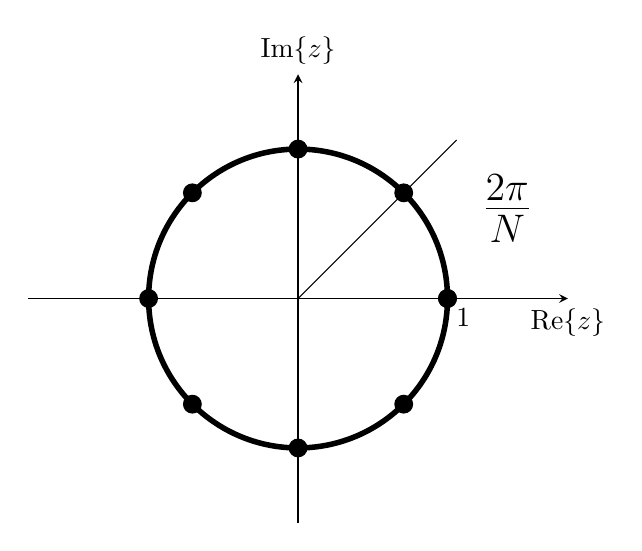
\begin{tikzpicture} 
\begin{axis}[
axis equal,
axis lines*=middle,
enlargelimits = false,
xmax=1.5,
xmin=-1.5,
ymin=-1.5,
ymax=1.5,
axis line style={->,>=stealth},
xlabel={$\mathrm{Re}\{z\}$},
ylabel={$\mathrm{Im}\{z\}$},
every axis x label/.style={
    at={(ticklabel* cs:1)},
    anchor=north,
},
every axis y label/.style={
    at={(ticklabel* cs:1)},
    anchor=south,
},
xtick={1},
ytick=\empty,
xticklabels={1},
%xmajorgrids,
%ymajorgrids,
xticklabel style = {xshift=+0.2cm},
every outer y axis line/.append style={white!15!black},
every y tick label/.append style={font=\color{white!15!black}},
legend style={draw=white!15!black,fill=white,legend cell align=left}]
%\pgfplotsinvokeforeach{0, 45,..., 360}{
%	\draw [black] (axis cs:0,0) -- (axis cs:{1.5*cos(#1)}, {1.5*sin(#1)});
%}
\draw [black] (axis cs:0,0) -- (axis cs:{1.5*cos(45)}, {1.5*sin(45)});
\draw[black, line width=2pt] (axis cs:0,0) circle [radius=1];
\draw [black, mark=*, mark size=3pt, only marks, thick,  domain=0:360, samples=9] plot ({cos(\x)}, {sin(\x)} );
%\draw[latex'-latex', double] (1.25,0) arc (0:45:1.25);
\node (z) at (axis cs: 1.4, 0.6) {\huge $\frac{2\pi}{N}$};
\end{axis}
\end{tikzpicture}
}
		\label{fig:sampled_unit_circle}
	\end{figure}
\end{frame}
